\section{Metrology in the vicinity of Dicke states}
\label{sec:vd}
\thiswatermark{\put(1,-282){\color{l-grey}\rule{84pt}{88pt}}
\put(84,-282){\color{grey}\rule{410pt}{88pt}}}


\quotes{Robert H. Dicke}{An experimentalist should not be unduely inhibited by theoretical untidyness}

\lettrine[lines=2, findent=3pt,nindent=0pt]{I}{n} this chapter we will present recent results regarding the metrological usefulness of a family of unpolarized states.
Such states can be used as prove states to estimate the homogeneous magnetic field strength, see Section~\ref{sec:bg-quantum-magnetometry} for references about magnetometry.
It turns out that the unpolarized states are the most adequate states to bite the Heisenberg limit, as it was shown on the Section~\ref{sec:bg-quantum-metrology}.
Hence, these states have attracted the interest of the community.

One of the figures of merit of this such unpolarized, but still useful, states is the so-called unpolarized Dicke state \citep{Dicke1954}, which consists of, on its $z$-axis  representation, an equal number of qubits pointing up and pointing down while the whole state is in the symmetric subspace.
It can be written as follows,
\be
  \ket{\dicke{N,\frac{N}{2}}} \equiv \ket{\dicke{N}}:= \binom{N}{N/2}^{-\frac{1}{2}}
  \sum_{k\in \sigma_\text{s}}
  \mathcal{P}_{k} \left( \ket{1}^{\otimes N/2} \ket{0}^{\otimes N/2}
  \right),
  \label{eq:vd-unpolarised-dicke}
\ee
where $k$ are elements of the set of all possible unique permutations of $N$ elements of 2 kinds, $\sigma_\text{s}$, see Appendix~{\ref{app:angular-subspaces}} for more information about this notation.
Such state is known to be highly entangled \citep{} and to reach Heisenberg scaling when used for magnetometry.

One of the most particular features this state has is that since it is a eigenstate of the collective operator $J_z$ with corresponding eigenvalue equal to zero.
At the same time, it lives in the subspace where the collective total spin is maximum, i.e, $\expect{\bs{J}^2}=N(N+2)/4$.
With this together with the fact that the state is unpolarized, it turns that it must have a very large uncertainty for the collective spin operators perpendicular to $J_z$, namely $J_x$ and $J_y$.

For metrology, we chose the $z$-axis to be parallel to the magnetic field.
Hence, the Dicke state should not be an eigenstate of $J_z$, it would not evolve in time making it useless for metrology, but an eigenstate of a perpendicular projection of the angular momentum operator such as $J_x$.
In this scheme, the state is rotated around the $z$-direction and the rotation angle must be estimated based on collective measurements.
For this case, a criterion to detect the metrological usefulness of some of these states has been derived for symmetric systems \citep{VD51}.

In this chapter, we present a condition for metrological usefulness for the case when the second moment of a total angular momentum component is measured to obtain an estimate for the rotation angle.
Our method is expected to simplify the experimental determination of metrological sensitivity since it is much easier to measure the collective operators of the state than carrying out the metrological procedure and measure directly the sensitivity.
We also test our approach using the experimental results of Refs.~\citep{VD48,VD50}, which realize parameter estimation with a Dicke state.
Thus, our work is expected to be useful for similar experiments in the future.

The chapter is organized as follows.
In Section~\ref{sec:vd-unpolarized-states-magnetometry}, we review some important concepts behind theory of metrology with unpolarized states.
In Section~\ref{sec:vd-evolution-of-the-expectation-values}, we present our criterion.
In Section~\ref{sec:vd-comparison-with-qfi}, we compare our result to sensitivity bounds obtained from the quantum Fisher information.
In Section~\ref{sec:vd-testing-with-experimental-data}, we show how to apply our criterion to experimental results.

\subsection{Unpolarized Dicke states for magnetometry}
\label{sec:vd-unpolarized-states-magnetometry}

The use of unpolarized states for magnetometry has been shown useful in Eq.~\eqref{eq:bg-unpolarize-states-are-better}.
While the quantum Fisher information would give us directly the performance one state would have, this is not feasible in general because a complete knowledge of the state is needed to compute such value, see Eq.~\eqref{eq:bg-qfi-definition-eigen-decomposition}.
On the other hand, we can use the error propagation formula Eq.~\eqref{eq:bg-error-propagation-formula} to obtain a bound on the achievable precision which at the same time bounds the QFI.

As one can see in Figure~\ref{fig:vd-secuence-evo}, a pure Dicke state of 16 qubits, initially an eigenstate of the $J_x$ operator, is rotated along the $z$-axis.
\begin{figure}[htp]
  \centering
  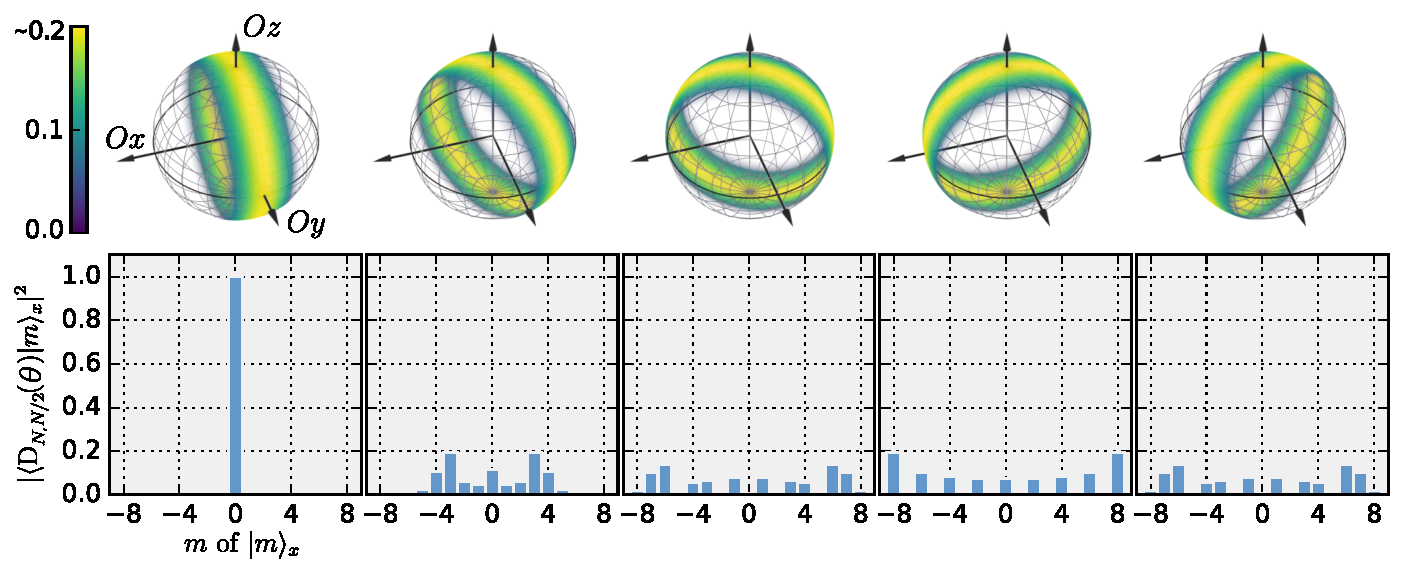
\includegraphics[scale=.65]{img/plots/VD_evolution_of_dicke.pdf}
  \caption[Sequence of Dicke state evolution]{Sequence of the evolution of an unpolarized Dicke state of 16 qubits for $\theta=\{i\pi/6\}_{i=0}^4$. Bloch spheres representing the Husimi quasi-probabilistic distribution of the state, and below PDF of the $J_x$ positive-operator valued measure (POVM) for each step of the sequence}
  \label{fig:vd-secuence-evo}
\end{figure}
The state is unpolarized so the expectation value of any component of the total angular momentum remains zero since the rotation of the system does not change that.
It turns out that measuring the evolution of the second statistical moment of $J_x$ is one of the ways to go.
The expectation value $\expect{J_x^2}$ will start having value equal to zero for a pure unpolarized Dicke state, and rapidly, it will increase its value as it can be seen in the Figure~\ref{fig:vd-secuence-evo}.
Another heuristic observation is that for $\theta=\pi/2$ the value of $\expect{J_x^2}$ will be at its maximum proportional to $\expect{\bs{J}^2}$ or equivalently to $\mathcal{J}_{N/2}$, see Eq.~\eqref{eq:app-maximum-total-angular-momentum}.
Hence, the change on the second moment over the phase shift must be in this case proportional to $N^2$.
We lead to the conclusion that one only needs to measure the second moment of the collective spin $J_x$ to achieve Heisenberg scaling for the estimation.

In certain situations, it is better to use Eq.~\eqref{eq:bg-error-propagation-formula} rather than Eq.~\eqref{eq:bg-cramer-rao-bound} for calculating the achievable precision, since it gives the precision for a particular operator to be measured in an experimental setup.
This is reasonable, since in a typical experiment, only a restricted set of operators can be measured.
In this work, we will consider many-particle systems in which the particles cannot be accessed individually, and only collective quantities can be measured.
As we said, measuring the second moment of $J_x$ is a valid choice to estimate the rotation angle.
In the following equation, we show the error propagation formula when measuring the second moment of the $J_x$ total angular momentum component,
\be
  \varinv{\theta} = \frac{|\partial_{\theta} \expect{J_x}|^2}{\varian{J_x^2}}.
  \label{eq:vd-error-propagation}
\ee

As a consequence of Eq.~\eqref{}, if
\be
  \frac{|\partial_{\theta} \expect{J_x}|^2}{\varian{J_x^2}}\geq N
\ee
holds, then the system is entangled.
Hence again, entanglement is required for a large metrological precision.
Based on Eq.~\eqref{}, we can find entanglement depth of the systems as follows.
Similarly to the previous paragraph, if for a quantum state
\be
  \frac{|\partial_{\theta} \expect{J_x}|^2}{\varian{J_x^2}}\geq kN
\ee
holds, then it is at least $(k+1)$-entangled.

\subsection{Evolution of the expectation values}
\label{sec:vd-evolution-of-the-expectation-values}
With the aim of computing the precision, Equation~{(\ref{eq:vd-error-propagation})}, we will compute the dependence on $\theta$ of the expectation value of the operator $J_x$ and higher order moments.
For that, first of all, we will move to the Heisenberg picture where the operators evolve in time while the state remains the same.
The operator $J_x$ can be written as a function of $\theta$ the following way,
\be
  J_x(\theta) = e^{i \theta J_z} J_x(0) e^{-i \theta J_z} = J_x(0) \text{c}_\theta - J_y(0) \text{s}_{\theta},
\ee
where $J_l(0)$ for $\forall l$ are the collective angular momentum operators at time equal zero, which we will write them simply $J_l$ from now on, and $\text{c}_\theta$ and $\text{s}_\theta$ are the trigonometric functions introduced on the first chapter.

We need to compute the second and the fourth moments of $J_x$ as it is required by the Equation~{(\ref{eq:vd-error-propagation})}.
But before any calculation we will make a simplifying assumption which turn to be well supported on the most common situations.
The assumption is that both expectation values are even functions on $\theta$,
\be
  \begin{split}
    \expect{J_x^2(\theta)} &=\expect{J_x^2(-\theta)}, \\
    \expect{J_x^4(\theta)} &=\expect{J_x^4(-\theta)}.
  \end{split}
  \label{eq:vd-even-f-constraint}
\ee

The square of $J_x$ in the Heisenberg picture is written as follows,
\be
  J_x^2(\theta)= J_x^2 \text{c}_\theta^2 + J_y^2 \text{s}_\theta^2
  - (J_xJ_y + J_yJ_x) \text{c}_\theta\text{s}_\theta.
\ee
From the equation above and to fulfill the first constraint on the Equation~{(\ref{eq:vd-even-f-constraint})} it turns out that the expectation value over our yet to be shown initial state of the operator $(J_xJ_y + J_yJ_x)$ must vanish.
Hence it is equivalent to the first assumption of the Equation~{(\ref{eq:vd-even-f-constraint})} write that
\be
  \expect{\{J_x,J_y\}} = 0
  \label{eq:vd-init-2nd-constraint}
\ee
where $\{\, ,\,\}$ stands for the anticommutator.
Apart for been simpler to compute the Equation~{(\ref{eq:vd-init-2nd-constraint})} is based also on initial expectation values of the state.
We will see that as we said before this is easily guarantied for most important cases.

As we have done recently with the square of $J_x$ now we will do it for $J_x^4$.
This way one will be able to distinguish which other combination of operators must vanish in order to have Equation~{(\ref{eq:vd-even-f-constraint})} guarantied. The fourth power of $J_x$ can be written as follows in the Heisenberg picture,
\begin{multline}
  J_x^4(\theta)= J_x^4 \text{c}_\theta^4 + J_y^4 \text{s}_\theta^4
  + (J_x^2J_y^2 + J_xJ_yJ_xJ_y + J_xJ_y^2J_x + J_yJ_xJ_yJ_x + J_yJ_x^2J_y + J_y^2J_x^2) \text{c}_\theta^2\text{s}_\theta^2 \\
  -(J_x^3J_y+J_x^2J_yJ_x+J_xJ_yJ_x^2+J_yJ_x^3)\text{c}_\theta^3\text{s}_\theta
  -(J_xJ_y^3+J_yJ_xJ_y^2+J_y^2J_xJ_y+J_y^3J_x)\text{c}_\theta\text{s}_\theta^3.
\end{multline}
And again assuming that its expectation value must be an even function on $\theta$ it turns out that the second line must be equal to zero when the expectation value is considered.
So $(J_x^3J_y+J_x^2J_yJ_x+J_xJ_yJ_x^2+J_yJ_x^3)$ and $(J_xJ_y^3+J_yJ_xJ_y^2+J_y^2J_xJ_y+J_y^3J_x)$ must vanish again over any candidate state to be used as prove state.
Hence, the second constraint of the Equation~{(\ref{eq:vd-even-f-constraint})} can be rewritten as follows,
\be
  \begin{split}
    \expect{\big\{J_x^2 , \{ J_x,J_y\}\big\}}=0,\\
    \expect{\big\{J_y^2 , \{ J_x,J_y\}\big\}}=0.
  \end{split}
\ee

Finally, we can write how the evolution of second and fourth moments of the $J_x$ operator must look like,
\begin{align}
  \expect{J_x^2(\theta)}=\; &\expect{J_x^2} \text{c}_\theta^2 + \expect{J_y^2} \text{s}_\theta^2
  \label{eq:vd-evo-2nd-moment}\\
  \begin{split}
    \expect{J_x^4(\theta)}=\; &
    \expect{J_x^4}\text{c}_\theta^4 + \expect{J_y^4} \text{s}_\theta^4 \\
    & + \expect{\{J_x^2,J_y^2\}+\{J_x,J_y\}^2} \text{c}_\theta^2\text{s}_\theta^2.
  \end{split}
\end{align}
From here we are able to write the evolution of the variance of the second moment when Equation~{(\ref{eq:vd-even-f-constraint})} must be obeyed.
We obtain
\be
  \begin{split}
    \varian{J_x^2(\theta)} &= \expect{J_x^4(\theta)} -\expect{J_x^2(\theta)}^2 \\
    &= \expect{J_x^4}\text{c}_\theta^4 + \expect{J_y^4} \text{s}_\theta^4
    + \expect{\{J_x^2,J_y^2\}+\{J_x,J_y\}^2} \text{c}_\theta^2\text{s}_\theta^2
    - \big(\expect{J_x^2} \text{c}_\theta^2 + \expect{J_y^2} \text{s}_\theta^2\big)^2\\
    &= \big(\expect{J_x^4}-\expect{J_x^2}^2\big)\text{c}_\theta^4
    + \big(\expect{J_y^4}-  \expect{J_y^2}^2\big)\text{s}_\theta^4
    + \big(\expect{\{J_x^2,J_y^2\}+\{J_x,J_y\}^2} - 2 \expect{J_x^2}\expect{J_y^2}\big)
    \text{c}_\theta^2\text{s}_\theta^2\\
    &=\varian{J_x^2}\text{c}_\theta^4 + \varian{J_y^2} \text{s}_\theta^4+ \big(\expect{\{J_x^2,J_y^2\}+\{J_x,J_y\}^2} - 2 \expect{J_x^2}\expect{J_y^2}\big)\text{c}_\theta^2\text{s}_\theta^2.
  \end{split}
\ee

The remaining constituent of the Equation~{(\ref{eq:vd-error-propagation})} on which we will base our result for the precision, is the modulus square of the derivative of the second moment of the $J_x$ operator.
Using Equation~{(\ref{eq:vd-evo-2nd-moment}) for the expression of the evolution of the second moment, the denominator of Equation~{(\ref{eq:vd-error-propagation})} follows
\be
  \begin{split}
    |\partial_\theta \expect{J_x^2(\theta)}|^2 & = |-2\expect{J_x^2}\text{c}_\theta\text{s}_\theta+2\expect{J_y^2}\text{c}_\theta\text{s}_\theta|^2\\
    & = 4\expect{J_y^2-J_x^2}^2\text{c}_\theta^2\text{s}_\theta^2.
  \end{split}
\ee

From the equations above directly follows expression for the precision of $\theta$,
\be
\begin{split}
  \varian{\theta} & = \frac{\varian{J_x^2}\text{c}_\theta^4 + \varian{J_y^2} \text{s}_\theta^4+ \big(\expect{\{J_x^2,J_y^2\}+\{J_x,J_y\}^2} - 2 \expect{J_x^2}\expect{J_y^2}\big)\text{c}_\theta^2\text{s}_\theta^2}
  {4\expect{J_y^2-J_x^2}^2\text{c}_\theta^2\text{s}_\theta^2}\\
  & = \frac{\varian{J_x^2}\text{t}_\theta^{-2} + \varian{J_y^2} \text{t}_\theta^2+ \expect{\{J_x^2,J_y^2\}+\{J_x,J_y\}^2} - 2 \expect{J_x^2}\expect{J_y^2}}
  {4\expect{J_y^2-J_x^2}^2}.
\end{split}
\label{eq:vd-result-before-simp}
\ee
To this calculations further computations follows mainly regarding to the following expectation value $\expect{\{J_x^2,J_y^2\}+\{J_x,J_y\}^2}$.
This calculus is left for the Appendix~{\ref{app:simplification-of-4th-moments}}.
Finally, the expression Equation~{(\ref{eq:vd-result-before-simp})} leads to the following,
\be
  \varian{\theta} = \frac{\varian{J_x^2}\text{t}_\theta^{-2} + \varian{J_y^2} \text{t}_\theta^2 + 4\expect{J_y^2} - 3 \expect{J_z^2} - 2\expect{J_x^2}(1+\expect{J_y^2}) + 6\expect{J_xJ_y^2J_x}}
  {4\expect{J_y^2-J_x^2}^2}
  \label{eq:vd-precision-as-theta}
\ee
[WOW IN THE PAPER FINALLY IT IS CORRECT!!]

We have verified the correctness of our analytical formula with a direct numeric simulation of the Equation~[ERROR PROP. FORM.] and the equation above.
For that we, have used the ground-state of $H=J_x^2+J_y$ for 6 qubits, $|\text{GS}\rangle$.
This state in principle does not have extra symmetries where further simplifications would take part on the final expression of the formula, so is more adequate for testing.
We have computed the evolution of the expectation values of the second and the fourth moments of the operator $J_x$ in the range of half a cycle, i.e, $\theta \in [0,\pi]$, for thousand of equidistant points.
We choose so high density of points on the range in order to compute a more accurate derivative of the expectation value $\partial_{\theta} \langle J_x^2\rangle$ appearing on the Equation~[EPF], see Figure~[REF]~(a).
Finally, we have also checked that the constraints assumed at the beginning of this section are fulfilled.
For that aim, the range of the evolution time has been $\theta \in [-\pi,\pi]$ and we have computed the expectation values for five hundreds of equidistant points, see Figure~[REF]~(b).
We can conclude saying that our formula exactly reproduces the evolution of the error propagation formula, Equation~[REF].
\begin{figure}[htp]
  \centering
  \igwithlabel{(a)}{scale=.65}{img/plots/VD_simulation.pdf}
  \igwithlabel{(b)}{scale=.65}{img/plots/VD_parity_simulation.pdf}
  \caption[(a) Evolution of $\theta$. (b) Evolution of expectation values]{(a) Evolution of the precision for 6 qubits based on the simulation of the system and its expectation values.
  The agreement with the Equation~[REF] is shown on the inset plot where the square of the difference between two approaches, the analytical and the simulation, is plotted.
  The difference is more or less two orders of magnitude below the actual value for the relevant points, which mainly comes because of the error coming from computing the derivative which has to be done approximately between two neighbor points.
  (b) Verification of the parity with respect to $\theta$ of the expectation values of the second and the fourth moment, so to fulfill the constraint Equation~[REF].}
  \label{fig:bg-histograms}
\end{figure}


\subsubsection{The optimal precision}
One can realize that the whole dependence on the phase shift is in the first two terms of the numerator.
This way one can minimize the sum on the first two terms in order to find where the precision is best.
So it follows that,
\be
  \tan^2(\theta_{\text{opt}}) = \sqrt{\frac{\varian{J_x^2}}{\varian{J_y^2}}}
\ee
which inserted on the Equation~{(\ref{eq:vd-precision-as-theta})} gives us the optimal precision when the second moment $\expect{J_x^2}$ is measured based on the initial expectation values of the input state. The optimal precision is written in the following way,
\be
  \varian{\theta}_{\text{opt}} = \frac{\sqrt{\varian{J_x^2} \varian{J_y^2} } + 4 \expect{J_y^2} - 3 \expect{J_z^2} - 2\expect{J_x^2}(1+\expect{J_y^2}) + 6\expect{J_xJ_y^2J_x}}
  {4\expect{J_y^2-J_x^2}^2}.
  \label{eq:vd-precision}
\ee.

We conclude with this section checking our bound for the pure unpolarised Dicke state aligned with the $x$-axis, $\ket{\text{D}_N}_x$, whose precision bound is well known, Equation~{([XXX])}.
With this aim we compute all the expectation values needed for the Equation~{(\ref{eq:vd-precision})} which almost all of them are trivial, $\expect{J_xJ_y^2J_x}=\expect{J_x^4}=\expect{J_x^2}=0$.
The rest are obtained in the following way,
\begin{align}
  \expect{J_y^2} & = \expect{J_z^2} = \frac{N (N+2)}{8},
  \label{eq:vd-2moment-pure-dicke}\\
  \expect{J_y^4} & = \frac{N+2}{8}\left(\frac{3N(N+2)}{16}-\frac{1}{2}\right).
  \label{eq:vd-4y-moment-pure-dicke}
\end{align}
The Equation~{(\ref{eq:vd-2moment-pure-dicke})} follows directly from the fact that the state is invariant under rotations on the $x$-axis, so they are its expectation values, because the sum of all the second moments must give the value of the total angular momentum, in this case the maximum which is $\expect{\bs{J}^2} = \frac{N (N+2)}{4}$, and because $\expect{J_x^2}=0$.
The proof of the Equation~{(\ref{eq:vd-4y-moment-pure-dicke})} needs more algebra and has been left for the Appendix~{\ref{ap:}}.

From the equations above, one lead to the following expression for the precision of the phase shift for a pure unpolarised Dicke state,
\be
  \varian{\theta} = \frac{2}{N(N+2)},
\ee
which coincides exactly with the inverse quantum Fisher information for such state.

\subsection{Testing the formula against some known states}
\label{sec:vd-comparison-with-qfi}

In this section we will compare our criteria based on few expectation values against the corresponding quantum Fisher information obtained for some known input states.
Those input states will be first the family of states defined as the ground states of the following Hamiltonian, called the spin-squeezing Hamiltonian,
\be
  H_\lambda = J_x^2 - \lambda J_y.
\ee
For $\lambda$ equal to zero we have the unpolarized Dicke state, Equation~{(\ref{eq:vd-unpolarised-dicke})}, and for $\lambda$ large we recover the coherent totally polarized state pointing onto the $y$-direction.
In the meantime the state is also a spin-squeezed state, therefore the name of the Hamiltonian.
The ground state is defined such that
\be
  \lambda_{\min} = \tr(H_\lambda \rho_\lambda),
\ee
where $\lambda_{\min}$ is the lowest eigenvalue of $H_\lambda$.
The state $\rho_\lambda$ is invariant under permutations of the particles and it is also pure.
Moreover the state $\rho_\lambda$ is symmetric.

The second family of input states we are going use are the Gaussian mixture of Dicke states around the unpolarized Dicke state, which have the following form as function of $\beta$,
\be
  \rho_{(T)} \propto \sum_{m=-N/2}^{N/2} e^{- \frac{m^2}{T}} \ket{\text{D}_N^m}_x\bra{\text{D}_N^m}_x.
\ee

\begin{figure}[htp]
  \centering
  \igwithlabel{(a)}{scale=.65}{img/plots/VD_against_spsq.pdf}
  \igwithlabel{(b)}{scale=.65}{img/plots/VD_against_therm.pdf}
  \caption[Bound against known QFIs for different states.]{Comparison between our formula for the precision and the QFI for different states. (a) Comparison for ground states of $H_\lambda$. (b) Comparison with gaussian mixture of Dicke states.}
  \label{fig:bg-histograms}
\end{figure}

After showing how the optimal precision formula behaves compared with the quantum Fisher information for those two families of states, we also have to proof that they indeed fulfill the constraints on Equation~{(\ref{eq:vd-even-f-constraint})}.

For the spin-squeezed state , $\rho_\lambda$, we have that it is invariant under

On the other hand for the thermal state, $\rho_T$, we have that it is invariant under rotations around the $x$-axis
\be
  \rho_T = e^{-i \alpha J_x} \rho_T e^{i \alpha J_x},
\ee
for arbitrary $\forall \alpha$.

\be
  \tr(e^{i\theta J_z}J_y^m e^{-i\theta J_z}\rho_T) = \tr(e^{i\theta J_z}J_y^m e^{-i\theta J_z} e^{-i \alpha J_x} \rho_T e^{i \alpha J_x})
\ee

If we choose $\alpha = \pi$ then we rotate all the orthogonal angular momentum operators such that $J_y \rightarrow - J_x$ and $J_z \rightarrow -J_z$.
Therefore, $e^{i \pi J_x}e^{i\theta J_z}J_y^m e^{-i\theta J_z} e^{-i \pi J_x}=e^{-i\theta J_z}(-J_y)^m e^{i\theta J_z}$.
Hence, for even $m$ and particularly for $m=2,4$ we have that,
\be
  \tr(e^{i\theta J_z}J_y^m e^{-i\theta J_z}\rho_T) = \tr(e^{-i\theta J_z}J_y^m e^{i\theta J_z}\rho_T ),
\ee
so the Equation~{(XXX)} is granted.

\subsection{Using our method with real experimental data}
\label{sec:vd-testing-with-experimental-data}

On reference [XXX], it is produced on the laboratory a state with the proper characteristics of an unpolarised Dicke state, small variance on one of the directions and very large one on the perpendicular directions to this.
It is also invariant under rotations around $x$-axis.
Effectively, the state has the following form,
\be
  \rho = \frac{1}{2\pi}\int e^{-i\alpha J_x} \rho_0 e^{i\alpha J_x},
\ee
where $\rho_0$is what we would obtain if we would have access to the phase reference.
Hence we have that at $\theta=0$ all the statistical moments $\expect{J_z^m}=\expect{J_y^m}$ are equal.

Simplification of our precision formula on Equation~{(XXX)}.
First, we simplify the expectation value $\expect{J_xJ_z^2J_x}$ in the following way,
\be
\begin{split}
  \expect{J_xJ_y^2J_x} &= \frac{\expect{J_x (J_y^2 + J_z^2)J_x}}{2}
  =\frac{\expect{J_x (J_x^2 + J_y^2 + J_z^2 )J_x} - \expect{J_x^4}}{2} \\
  & \leq \frac{N(N+2)}{8} \expect{J_x^2} - \frac{\expect{J_x^4}}{2}.
\end{split}
\ee
Notice that obtaining $\expect{J_xJ_z^2J_x}$ is hard experimentally.
This simplification can only make our estimation of the precision worse while for symmetric states the equality holds.
The bound from below for the precision can be writtes as,
\be
  \varian{\theta}_{\text{opt}} \leq \frac{\sqrt{\varian{J_x^2} \varian{J_y^2} } + \expect{J_y^2} + \frac{3N(N+2)-8}{4} \expect{J_x^2} - 2\expect{J_x^2}\expect{J_y^2} - 3\expect{J_x^4}}
  {4\expect{J_y^2-J_x^2}^2},
\ee
where some terms were reordered and further simplified.

It is worth to study this case and apply our methods such that we can extract conclusions about the metrological usefulness of the state.
The system in consideration is a $N=7900$ particles system.
The measured data for such system is
\be
\begin{aligned}
  \expect{J_x^2} & = 112 \pm 31, \\
  \expect{J_x^4} & = 40 \times 10^3 \pm 22 \times 10^3,
\end{aligned}
\quad
\begin{aligned}
  \expect{J_y^2} & = 6 \times 10^6 \pm 0.6 \times 10^6, \\
  \expect{J_y^4} & = 6.2 \times 10^{13} \pm 0.8 \times 10^{13}.
\end{aligned}
\ee
Hence we obtain the maximum precision,
\be
  \frac{(\Delta \theta)^{-2}_{\text{opt}}}{N} \geq 3.7 \pm 1.5
\ee
with boot straping methods.
The direct substitution would yield to a 3.3 gain over the shot-noise limit.

Next we plot the value for the precision substituting directly the measured data into Equation~{(XXX)}, see Figure~\ref{fig:vd-precision-theta}.
\begin{figure}[htp]
  \centering
  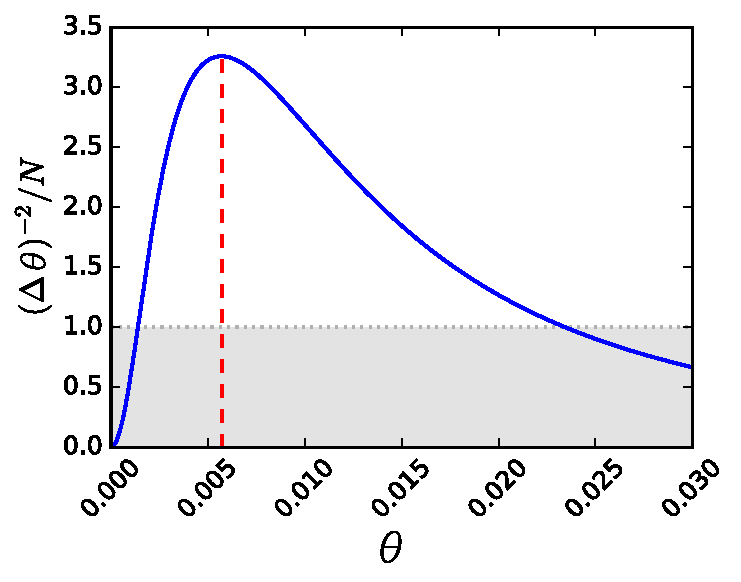
\includegraphics[scale=.65]{img/plots/VD_precision_theta.pdf}
  \caption[Evolution of the precision for $\theta$.]{The (solid) line shows how the precision of $\theta$ varies through the evolution. Notice that for the initial moment the precision is zero and that it reaches a maximum at $\theta \approx 0.0057$ highlighted with the vertical (dashed) line. The gray area represent the region where the precision is below the shot-noise limit.}
  \label{fig:vd-precision-theta}
\end{figure}

Further simplification of our method can be achieved for states of the kind of the one studied on this section.
Based on $\expect{AB}\leq\lambda_{\max}(A)\expect{B}$ for two commuting positive-semidefinite observables,
\be
  \expect{J_y^4}\leq\frac{N^2}{4}\expect{J_x^2}.
\ee

We can also approximate $\expect{J_x^4}$ with $\expect{J_x^2}$ in the sense that it is small and that mainly its value comes from technical noise,
\be
  \expect{J_x^4} \approx \beta \expect{J_x^2}^2.
\ee
This approximation even if it is not a strict bound on the precision can be very useful in order to characterize the metrological usefulness of our input state based only on second statistical moments of only two angular momentum operators, namely $\expect{J_z^2}$ and $\expect{J_x^2}$.
Those two expectation values are related with the width of our state and also with how thin we can do it in one of the directions, for metrological purposes, perpendicular to the magnetic field.
So in this case we use $\beta=3$ assuming that the distribution function has Gaussian shape.

From these considerations we are able to write a second bound with fewer expectation values for the optimal precision such that,
\be
  \varian{\theta}_{\text{opt}} \leq \frac{\expect{J_y^2} + \frac{3N(N+2)-8}{4} \expect{J_x^2} + \Big(\sqrt{\frac{N^2}{2\expect{J_y^2}}-2} - 2 \Big) \expect{J_y^2}\expect{J_x^2} - 9\expect{J_x^2}^2}
  {4\expect{J_y^2-J_x^2}^2}.
\ee
We have used this formula to compute the bound on the optimal precision with the measured data shown on Equation~{(XXX)}, $(\Delta \theta)^{-2}_{\text{opt}} \geq 2.9N$, see Figure~{\ref{fig:vd-experimental}}.

\begin{figure}[htp]
  \centering
  \igwithlabel{(a)}{scale=.65}{img/plots/VD_exper_contour.pdf}
  \igwithlabel{(b)}{scale=.65}{img/plots/VD_exper_slice.pdf}
  \caption[(a) Region of precision and experimental data. (b) Constant $\expect{J_y^2}$ section.]{Comparison between our formula for the precision and the QFI for different states. a) Comparison for ground states of $H_\lambda$. (b) Comparison with gaussian mixture of Dicke states.}
  \label{fig:vd-experimental}
\end{figure}
